\documentclass{beamer}
\usetheme{Dresden}
\usecolortheme{dolphin}

\usepackage[T1]{fontenc}
\usepackage[utf8]{inputenc}
\usepackage[british]{babel}
\usepackage{amsmath}
\usepackage{amsthm}
\usepackage{graphicx}
\usepackage{epstopdf}
\usepackage{subfig}
\usepackage{caption}
\captionsetup{skip=0pt, belowskip=0pt}
\captionsetup[figure]{labelformat=empty}
\setbeamerfont{caption}{size=\scriptsize}

\usepackage{pgfplots}
\pgfplotsset{every tick label/.append style={font=\tiny}}
\usepackage{animate}
\usepackage{bbm}
\usepackage{booktabs}
\usepackage{wrapfig}

\setbeamercovered{transparent}

\graphicspath{{img/}}

\title
[DG-FE approximations of elliptic problems of polyhedral grids]
{Discontinuous Galerkin Finite Element approximations of elliptic problems on 
polyhedral grids}
\author[Andrea Vescovini]{Andrea Vescovini\\ Supervisor: Prof. P. Antonietti}
\institute{Politecnico di Milano}
\date{1st December 2017}
%%%%%%%%%%%%%%%%%%%%%%%%%%%%%%%%%%%%%%%%%%%%%%%%%%%%%%%%%%%%%%%%%%%%%%%%%%%%
\begin{document}
\begin{frame}
	\centering
	%\includegraphics[scale=0.5]{logo}
	\maketitle
\end{frame}
%%%%%%%%%%%%%%%%%%%%%%%%%%%%%%%%%%%%%%%%%%%%%%%%%%%%%%%%%%%%%%%%%%%%%%%%%%%%
\begin{frame}
	\tableofcontents
\end{frame}
%%%%%%%%%%%%%%%%%%%%%%%%%%%%%%%%%%%%%%%%%%%%%%%%%%%%%%%%%%%%%%%%%%%%%%%%%%%%
\section[DG methods]{Discontinuous Galerkin methods}
\begin{frame}{Model problem}
	Poisson problem with Dirichlet boundary conditions:
	\begin{align} \label{eq:poisson}
	-\Delta u = f & \mbox{ in } \Omega\\
	u = g & \mbox{ on } \partial \Omega
	\end{align}	
\end{frame}
%%%%%%%%%%%%%%%%%%%%%%%%%%%%%%%%%%%%%%%%%%%%%%%%%%%%%%%%%%%%%%%%%%%%%%%%%%
\begin{frame}{Variational formulation}
	cont
\end{frame}
%%%%%%%%%%%%%%%%%%%%%%%%%%%%%%%%%%%%%%%%%%%%%%%%%%%%%%%%%%%%%%%%%%%%%%%%%%%
\section{Implementation details}
\begin{frame}{Basis functions}
	\begin{itemize}
		\item $\forall \kappa \in \mathcal{T}$ construct a cartesian bounding 
		box $B_\kappa=I_1\times I_2 \times I_3$.
		\item Define $\mathbb{P}_r(B_\kappa)$ spanned by basis 
		functions $\{ \phi_{i,\kappa} \}_{i=1}^{dim(\mathbb{P}_r(B_\kappa))}$.
	\end{itemize}
	We choose tensor product (scaled) Legendre polynomials:
	\begin{equation*}
	L_r^{[I_b]} (x) = \frac{1}{\sqrt{h_b}} L_r \bigg( \frac{x-m_b}{h_b} \bigg), 
	\quad h_b = \frac{x_2-x_1}{2}, \quad m_b=\frac{x_1+x_2}{2}.
	\end{equation*}
	The basis over $B_\kappa$ is:
	\begin{equation*}
	\phi_{\kappa,i}(\mathbf{x}) = 
	L_{r_1}^{[1]}(x)L_{r_2}^{[2]}(y)L_{r_3}^{[3]}(z), \quad
	r_1+r_2+r_3 \leq r, \quad r_k \geq 0, \quad k = 1,2,3.
	\end{equation*}
	\begin{itemize}
		\item Restrict the support of $\phi_{\kappa, i}(\mathbf{x}), \; 
		i=1,\dots,dim(\mathbb{P}_r(B_\kappa))$ to $\kappa$.
	\end{itemize}
\end{frame}
%%%%%%%%%%%%%%%%%%%%%%%%%%%%%%%%%%%%%%%%%%%%%%%%%%%%%%%%%%%%%%%%%%%%%%%%%%%
\begin{frame}{Matrix assembly}
	We expand the solution $u_h$ in basis functions and we get the 
	algebraic formulation: find $\mathbf{u} = [u_1, \dots, u_{N_h}]^T \in 
	\mathbb{R}^{N_h} $ such that:
	\begin{equation*}
	\mathrm{A}\mathbf{u} = \mathbf{f},
	\end{equation*}
	where $\mathrm{A} \in \mathbb{R}^{N_h \times N_h}, \; \mathrm{A}_{ij} = 
	a(\phi_j, \phi_i)$ and $\mathbf{f} \in \mathbb{R}^{N_h}, \; \mathbf{f}_i = 
	F(\phi_i)$.\\
	\vspace*{0.4cm}
	The matrix $\mathrm{A}$ is the sum of four matrices $\mathrm{A} = 
	\mathrm{V} - \mathrm{I} - \mathrm{I}^T + \mathrm{S}$:\\
	\begin{itemize}
		\item $\mathrm{V}_{ij} = \sum\limits_{\kappa \in \mathcal{T}} 
		\int_\kappa 
		\nabla \phi_j \cdot \nabla \phi_i, \quad i,j=1,\dots,N_h$
		\item $\mathrm{I}_{ij} = \sum\limits_{e \in \Gamma} \int_e 
		[\![\phi_j]\!] 
		\cdot \{\!\!\{ \nabla \phi_i \}\!\!\}, \quad i,j=1,\dots,N_h$
		\item $\mathrm{S}_{ij} = \sum\limits_{e \in \Gamma} \gamma_e \int_e 
		[\![ 
		\phi_j ]\!] \cdot [\![ \phi_i ]\!], \quad i,j=1,\dots,N_h$
	\end{itemize}
\end{frame}
%%%%%%%%%%%%%%%%%%%%%%%%%%%%%%%%%%%%%%%%%%%%%%%%%%%%%%%%%%%%%%%%%%%%%%%%%%%
\begin{frame}{Sparsity pattern}
	\vspace*{-12pt}
	\begin{align*}
	\mathrm{I} \rightarrow \int_e [\![\phi_j]\!] \cdot \{\!\!\{ \nabla \phi_i 
	\}\!\!\} &=
	\frac{1}{2} \int_e (\nabla{\phi_i}^+ \cdot \mathbf{n}^+ )\phi_j^+
	+ \frac{1}{2} \int_e (\nabla{\phi_i}^- \cdot \mathbf{n}^- )\phi_j^-\\
	&- \frac{1}{2} \int_e (\nabla{\phi_i}^+ \cdot \mathbf{n}^+ )\phi_j^-
	- \frac{1}{2} \int_e (\nabla{\phi_i}^- \cdot \mathbf{n}^- )\phi_j^+
	\end{align*}
	\vspace*{-1cm}
	\begin{minipage}[t]{0.55\textwidth}
		\begin{multline*}
			\mathrm{S} \rightarrow \gamma_e \int_e [\![\phi_j]\!] \cdot 
			[\![\phi_i]\!] =\\
			\gamma_e \int_e \phi_i^+ \phi_j^+
			+ \gamma_e \int_e \phi_i^- \phi_j^-\\
			- \gamma_e \int_e \phi_i^+ \phi_j^-
			- \gamma_e \int_e \phi_i^- \phi_j^+
		\end{multline*}
	\end{minipage}%%%%%%%%%%%%%%%%
	\begin{minipage}[t]{0.45\textwidth}
	\begin{figure}
		\centering
		\includegraphics[scale=0.35]{spy_A}\\
		\tiny
		\textit{Sparsity pattern of $\mathrm{A}$ computed over a mesh 
		of 392 polyhedral elements and $r=2$}.
	\end{figure}
\end{minipage}
\end{frame}
%%%%%%%%%%%%%%%%%%%%%%%%%%%%%%%%%%%%%%%%%%%%%%%%%%%%%%%%%%%%%%%%%%%%%%%%%%%
\begin{frame}{Quadrature rules}
	\begin{itemize}
		\item Construct a sub-triangulation.
		\item Exploit standard integration schemes.
	\end{itemize}
	For example let	$\kappa_\mathcal{S} = \{\tau_\kappa\}$ be a non-overlapping 
	sub-triangulation for the element $\kappa$ made of tetrahedra:
	\begin{multline*}
	\int_\kappa \nabla u \cdot \nabla v = \sum_{\tau_\kappa \in 
	\kappa_\mathcal{S}} \nabla u \cdot \nabla v \approx\\
	\approx \sum_{\tau_\kappa \in 
	\kappa_\mathcal{S}} \sum_{i=1}^{q} \nabla u(F_\kappa(\xi_i)) \cdot \nabla 
	v(F_\kappa(\xi_i)) det(J_{F_\kappa}(\xi_i))w_i,
	\end{multline*}
	where $F_\kappa: \hat{\kappa} \rightarrow \tau_\kappa$ is the map from the 
	reference simplex $\hat{\kappa}$ to $\tau_\kappa$ and $(\xi_i, 
	w_i)^q_{i=1}$ denote the quadrature nodes and weights 
	over $\hat{\kappa}$.
\end{frame}
%%%%%%%%%%%%%%%%%%%%%%%%%%%%%%%%%%%%%%%%%%%%%%%%%%%%%%%%%%%%%%%%%%%%%%%%%%%
\section{Numerical results}
\begin{frame}{Numerical results}
	We test the method choosing $\Omega = (0,1)^3$, $u(x,y,z) = e^{xyz}$, $\sigma = 10$.
	\begin{figure}
		\centering
	%	\subfloat[\textit{Solution computed over a polyhedral mesh.}]
		\subfloat[Solution computed over a polyhedral mesh.]
		{\includegraphics[width=.45\textwidth]{solution_3072p}}
		\quad
	%	\subfloat[\textit{Polyhedral mesh consisting of 15 elements.}]
		\subfloat[Polyhedral mesh consisting of 15 elements.]
		{\includegraphics[width=.45\textwidth]{mesh_48p}}
	\end{figure}
\end{frame}
%%%%%%%%%%%%%%%%%%%%%%%%%%%%%%%%%%%%%%%%%%%%%%%%%%%%%%%%%%%%%%%%%%%%%%%%%%%%
\begin{frame}{$h$-convergence}
	\begin{itemize}
		\item Tetahedral, hexahedral, mixed tetrahedral/hexahedral and 
		polyhedral meshes.
		\item $r = 1,2,3$.
		\item $L^2$-norm and $H^1$-seminorm of the error $e_h = u - u_h$.
	\end{itemize}
	
	\begin{table} \tiny
		\centering
		\[
		\begin{array}{ccccccc}
		\toprule
		r & Error & \text{28 elem} & \text{224 elem} & \text{756 elem} & 
		\text{1792 elem} & \text{Rate} \\ 
		\midrule
		2 & |\!|\nabla e_{h}|\!|_{L^2} & 7.4183 \times 10^{-2} & 1.9944 \times 
		10^{-2} & 8.9959 \times 10^{-3} & 5.0984 \times 10^{-3} & 1.9738\\
		& |\!|e_{h}|\!|_{L^2} & 4.1276 \times 10^{-3} & 7.0478 \times 10^{-4} & 
		2.1079 \times 10^{-4} & 
		8.9470 \times 10^{-5} & 2.9787\\
		\bottomrule
		\end{array}
		\]
		\caption{\textit{Computed errors on a sequence of mixed 
		tetrahedral/hexahedral meshes.}}
%	\end{table}
%\begin{table} \tiny
%	\centering	
	\[
	\begin{array}{ccccccc}
	\toprule
	r & Error & \text{15 elem} & \text{120 elem} & \text{392 elem} & 
	\text{965 elem} & \text{Rate} \\ 
	\midrule
	2 & |\!|\nabla e_{h}|\!|_{L^2} & 8.7963 \times 10^{-2} & 4.2298 \times 
	10^{-2} & 2.3058 \times 10^{-2} & 1.3036 \times 10^{-2} & 1.9823\\
	& |\!|e_{h}|\!|_{L^2} & 5.3520 \times 10^{-3} & 1.8324 \times 10^{-3} & 
	7.5865 \times 10^{-4} & 2.8963 \times 10^{-4} & 3.3472\\
	\bottomrule
	\end{array}
	\]
	\caption{\textit{Computed errors on a sequence of polyhedral meshes..}} 
\end{table}
	
\end{frame}
%%%%%%%%%%%%%%%%%%%%%%%%%%%%%%%%%%%%%%%%%%%%%%%%%%%%%%%%%%%%%%%%%%%%%%%%%%%
\begin{frame}{Comparison with other methods}
	Comparison with:
	\begin{itemize}
		\item classical SIPG method, based on a Lagrange polynomial basis.
		\item standard continuous Galerkin finite element method.
	\end{itemize}
\end{frame}
%%%%%%%%%%%%%%%%%%%%%%%%%%%%%%%%%%%%%%%%%%%%%%%%%%%%%%%%%%%%%%%%%%%%%%%%%%
\begin{frame}{$r$-convergence}
	\begin{itemize}
		\item Tetahedral, hexahedral, mixed tetrahedral/hexahedral and 
		polyhedral meshes.
		\item $r = 1,2,3$.
		\item $L^2$-norm and $H^1$-seminorm of the error $e_h = u - u_h$.
	\end{itemize}
	\vspace*{-0.7cm}
	\begin{figure}
		\subfloat[Tet/hex elements.]{
			\begin{tikzpicture}
			\begin{semilogyaxis}[width=0.55\textwidth, height=0.55\textheight, 
			xlabel style={font=\tiny}, xlabel={Basis degree}, xtick={1,2,3}, 
			legend style={font=\tiny}]
			\addplot coordinates
			{(1, 9.4090e-2) (2, 5.0984e-3) (3, 2.7689e-4)};
			\addlegendentry{$|\!|\nabla e_{h}|\!|_{L^2}$}	
			\addplot coordinates
			{(1, 1.4851e-3) (2, 8.9470e-5) (3, 3.9958e-6)};
			\addlegendentry{$|\!|e_{h}|\!|_{L^2}$}
			%	\legend{$|\!|\nabla e_{h}|\!|_{L^2}$, $|\!|e_{h}|\!|_{L^2}$}
			\end{semilogyaxis}
			\end{tikzpicture}}
		\subfloat[Polyhedral elements.]{
			\begin{tikzpicture}
			\begin{semilogyaxis}[width=0.55\textwidth, height=0.55\textheight, 
			xlabel style={font=\tiny}, xlabel={Basis degree}, 
			xtick={1,2,3}, legend style={font=\tiny}]
			\addplot coordinates
			{(1, 1.4168e-1) (2, 1.3036e-2) (3, 1.1137e-3)};
			\addlegendentry{$|\!|\nabla e_{h}|\!|_{L^2}$}	
			\addplot coordinates
			{(1, 5.9973e-3) (2, 2.8963e-4) (3, 2.0407e-5)};
			\addlegendentry{$|\!|e_{h}|\!|_{L^2}$}
			\end{semilogyaxis}
			\end{tikzpicture}}
	\end{figure}
\end{frame}
%%%%%%%%%%%%%%%%%%%%%%%%%%%%%%%%%%%%%%%%%%%%%%%%%%%%%%%%%%%%%%%%%%%%%%%%%%%
\begin{frame}{$r$-convergence}
	\vspace*{-0.5cm}
	\begin{figure}[h]
		\centering
		\subfloat[][Tetrahedral elements.]{
			\begin{tikzpicture}
			\begin{semilogyaxis}[width=0.55\textwidth, height=0.4\textheight, 
			xlabel near ticks, xlabel style={font=\tiny}, xlabel={Basis 
				degree}, xtick={1,2,3}, 
			legend style={font=\tiny}]
			\addplot coordinates
			{(1, 9.9471e-2) (2, 4.6327e-3) (3, 2.0627e-4)};
			\addlegendentry{$|\!|\nabla e_{h}|\!|_{L^2}$}	
			\addplot coordinates
			{(1, 1.0227e-3) (2, 9.4460e-5) (3, 3.6715e-6)};
			\addlegendentry{$|\!|e_{h}|\!|_{L^2}$}
			\end{semilogyaxis}
			\end{tikzpicture}}
		\subfloat[][Hexahedral elements.]{
			\begin{tikzpicture}
			\begin{semilogyaxis}[width=0.55\textwidth, height=0.4\textheight, 
			xlabel near ticks, xlabel style={font=\tiny}, xlabel={Basis 
				degree}, 
			xtick={1,2,3}, 
			legend style={font=\tiny}]
			\addplot coordinates
			{(1, 8.4123e-2) (2, 4.6362e-3) (3, 2.5782e-4)};
			\addlegendentry{$|\!|\nabla e_{h}|\!|_{L^2}$}	
			\addplot coordinates
			{(1, 1.8931e-3) (2, 7.9122e-5) (3, 3.6604e-6)};
			\addlegendentry{$|\!|e_{h}|\!|_{L^2}$}
			\end{semilogyaxis}
			\end{tikzpicture}}\\
		\vspace*{-0.4cm}
		\subfloat[][Tet/hex elements.]{
			\begin{tikzpicture}
			\begin{semilogyaxis}[width=0.55\textwidth, height=0.4\textheight, 
			xlabel near ticks, xlabel style={font=\tiny}, xlabel={Basis 
			degree}, 
			xtick={1,2,3}, 
			legend style={font=\tiny}]
			\addplot coordinates
			{(1, 9.4090e-2) (2, 5.0984e-3) (3, 2.7689e-4)};
			\addlegendentry{$|\!|\nabla e_{h}|\!|_{L^2}$}	
			\addplot coordinates
			{(1, 1.4851e-3) (2, 8.9470e-5) (3, 3.9958e-6)};
			\addlegendentry{$|\!|e_{h}|\!|_{L^2}$}
			\end{semilogyaxis}
			\end{tikzpicture}}
		\subfloat[][Polyhedral elements.]{
			\begin{tikzpicture}
			\begin{semilogyaxis}[width=0.55\textwidth, height=0.4\textheight, 
			xlabel near ticks, xlabel style={font=\tiny}, xlabel={Basis 
				degree}, xtick={1,2,3}, 
			legend style={font=\tiny}]
			\addplot coordinates
			{(1, 1.4168e-1) (2, 1.3036e-2) (3, 1.1137e-3)};
			\addlegendentry{$|\!|\nabla e_{h}|\!|_{L^2}$}	
			\addplot coordinates
			{(1, 5.9973e-3) (2, 2.8963e-4) (3, 2.0407e-5)};
			\addlegendentry{$|\!|e_{h}|\!|_{L^2}$}
			\end{semilogyaxis}
			\end{tikzpicture}}
		\label{fig:rconv}
	\end{figure}
\end{frame}
%%%%%%%%%%%%%%%%%%%%%%%%%%%%%%%%%%%%%%%%%%%%%%%%%%%%%%%%%%%%%%%%%%%%%%%%%%%%%%%%
\begin{frame}{Main references}
\begin{itemize}
	\item Antonietti, Houston, Hu, Sarti, Verani: Multigrid 
	algorithms for hp-version interior penalty discontinuous Galerkin methods 
	on polygonal and polyhedral meshes, \emph{Calcolo}, (2017).
	\item Cangiani, Georgoulis, Houston: Hp-Version discontinuous 
	Galerkin methods on polygonal and polyhedral meshes, \emph{Mathematical 
		Models and Methods in Applied Sciences} (2014).
	\item Quarteroni: \emph{Numerical Models for Differential Problems}, Springer (2014).
	\item Rivière: \emph{Discontinuous Galerkin Methods for Solving Elliptic and 
		Parabolic Equations: Theory and Implementation}, SIAM (2008).
\end{itemize}
\end{frame}
\end{document}